\documentclass[12pt]{article}
\usepackage[utf8x]{inputenc}
\usepackage[margin=0.75in]{geometry}

\usepackage{natbib}
\usepackage{color}
\usepackage{graphicx}
\usepackage{xcolor}
\usepackage{wrapfig}
\usepackage{hyperref}
\definecolor{lblue}{rgb}{0,0.41,0.49}


\renewcommand{\baselinestretch}{1.1} 


\usepackage{titling}

\setlength{\droptitle}{-2.5cm}

\begin{document}
\title{Research and Service}
\author{Thomas Gilray}
\date{}
\maketitle
\vspace{-1.25cm}
\small

\paragraph{Research Summary}

My research develops \textbf{high-performance programming-language approaches to reasoning automatically about complex systems}. I publish my work at top venues in programming languages (POPL, ICFP, JFP, PLDI, and ASPLOS), databases (VLDB), artificial intelligence (AAAI), and high-performance computing (HPDC, ICS, ISC, HiPC, and CLUSTER), aiming to bridge the gap between human-level formal systems (such as natural-deduction-style abstract interpreters and type systems) and their implementation in terms of lower-level data-parallel constructs (such as relational algebra and sparse linear algebra), addressing key performance and expressivity concerns that span the full system stack. My research focuses particularly on developing rich auto-tunable program analyses, strategies for declarative specification of such analyses, programming-language paradigms for deduction and chain-forward reasoning, and high-performance-computing algorithms to support scaling and parallelizing these tasks.


\paragraph{Research Support}

I have applied these approaches in a collaborative project with Galois, inc., starting in 2021, with a goal to develop scalable whole-component analyses that can serve applications in automated program repair---\textbf{work funded via a DARPA VSPELLS grant} (awarding us \$8M over 4 years, \textbf{\$400K of which funds my group} through a subcontract). This collaboration has yielded advances in program-analysis design and implementation, and lead to an open-source pointer-analysis framework for LLVM, called Yapall\footnote{\url{https://github.com/GaloisInc/yapall}}, written in Rust using a procedural-macro-based Datalog\footnote{\url{https://s-arash.github.io/ascent/}}.
Over the last few years, work in these directions have lead me to invest in promising collaborations with like-minded researchers at several other universities.
In 2022, \textbf{I lead a team of three PIs to successfully win an NSF PPoSS Planning} grant (Principles and Practice of Scalable Systems: awarding us \$250K over 1 year---\textbf{\$83K of which is awarded to my lab}). Leveraging this funding, collaborators and I made key breakthroughs in scaling parallel multi-node iterated joins and in extending the expressivity of Datalog for the purposes of program analysis (detailed further below). 
In 2023, \textbf{I lead a team of seven PIs to successfully win an NSF PPoSS Large} grant (awarding us \$5M over 5 years---\textbf{\$1.05M of which is awarded to my lab}) based on a shared vision of how to enable next-generation automated-reasoning tasks to scale effectively on supercomputers and HPC clouds.
In 2025, \textbf{I helped to win an ARPA-H grant} in collaboration with precision-medicine researchers in Colorado and Alabama, to study secure deductive databases for electronic health records: awarding us \$10M over 5 years---\textbf{\$1.29M of which is awarded to my lab}. I have also been supported by the Argonne Leadership Computing Facility (ALCF) director's discretion program and have utilized \textbf{over 5M compute hours} on the Theta supercomputer through this program.   


\paragraph{Research Vision}

Effective programming languages permit their users to write high-performance code in a manner that is as close to the form of their own thinking as possible. 
A long-standing dream in the area of programming languages been to \textbf{develop especially high-level \emph{declarative} languages that help to bridge this gap between \emph{specification} and \emph{implementation}}. Declarative programming permits a user to provide a set of high-level rules and declarations that offer the sought-after solution as a latent implication to be materialized automatically by the computer. 
The semantics of a declarative language does the heavy lifting in operationalizing this specification for a target computational substrate---one with its own low-level constraints and biases. 
Modern computers provide many threads of parallel computation, may be networked to further increase available parallelism, and are increasingly virtualized within ``cloud'' services. 
The complexity of next-generation \emph{exascale} systems pose new challenges: managing increased parallelism, heterogeneity, GPUs, and deep memory hierarchies. With this increasing complexity and diversity in the hardware configuration of upcoming HPC systems, it becomes very challenging to write high-performing scalable applications by hand.
The future of high-performance declarative programming languages \textbf{must refine their suitability on both sides of this gulf: becoming both more tailored to human-level reasoning and to modern, massively-parallel, GPU-accelerated, multi-node machines}, interposing an intelligent, fully-automated, generative pipeline between.


\paragraph{A Full-Stack Approach}

\begin{wrapfigure}{r}{3.45in}
\vspace{-0.85cm}
\centering
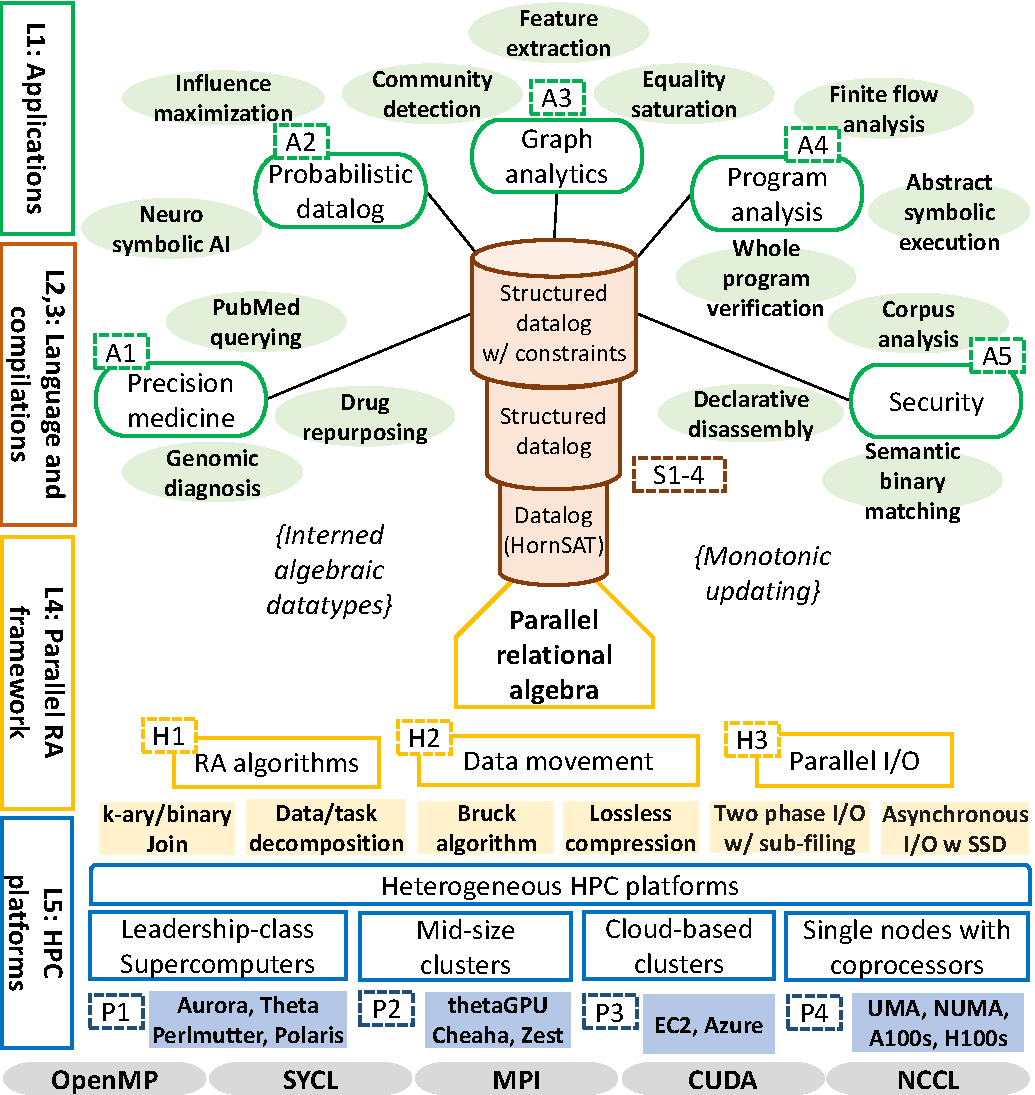
\includegraphics[width=3.45in]{PPoSS_Tree.pdf}
\vspace{-.9cm}
\caption{\footnotesize Concept tree for my PPoSS Large project}
\vspace{-0.55cm}
\end{wrapfigure}
%
My full-stack research program is illustrated as a concept tree. 
Application foci (leaves), forming five broad areas (\textbf{A1}-\textbf{A5}) ranging from medicine to security, branch off a trunk of higher-order, declarative, chain-forward programming languages leveraging heterogeneous, high-performance implementations (roots).

My research aims to support declarative analytics for applications from a range of domains while balancing \emph{performance} versus \emph{expressivity}, and maintaining \emph{correctness}. While my declarative \textsc{Slog} language\footnote{\url{https://github.com/harp-lab/slog-lang1}} (Structured Datalog) provides a highly expressive medium, my work on tunable and scalable relational-algebra frameworks supports performance through data-parallel evaluation using MPI and GPU accelerators. My end-to-end system spans a full stack of abstraction layers with a variety of key concerns that cut across multiple layers, requiring thoughtful co-design.

For example, at the application layer (\textbf{L1}), I am exploring medical applications, including reasoning over knowledge graphs for PubMed querying and for drug repurposing (\textbf{A1}-\textbf{A3}) in collaboration with the Precision-Medicine Institute at the University of Alabama at Birmingham, and exploring privacy-preserving deductive databases for electronic health records with the Barbara Davis Center at the University of Colorado. I am also applying my primary background in program analysis (\textbf{A4}) to security-relevant analyses and reverse engineering (\textbf{A5}) with collaborators here at WSU and at Syracuse University. Techniques required for probabalistic Datalog (\textbf{A2}) and higher-order analysis augmented with symbolic execution (\textbf{A4}) require key extensions to the declarative language (\textsc{Slog}) I'm developing (\textbf{L2})---notably first-class facts with lattice measurements---which must be supported in the compiler (\textbf{L3}), down through to the implementation layer (\textbf{L4}). This must then be supported by platform-level concerns (\textbf{L5}), such as data-movement algorithms (\textbf{H2}) and scheduling that must work differently on clusters (\textbf{P1}) versus GPUs (\textbf{P2},\textbf{P4}).

My central goal is to develop and extend high-performance primitives for reasoning (especially data-parallel operations on relational data, \textbf{H1}) all the way up human-level formal reasoning. A user should be able to transliterate standard, \LaTeX-rendered natural-deduction-style reasoning, as used in type systems, formal methods, and program analysis (\textbf{A4},\textbf{A5}) or semantic-web search (\textbf{A1},\textbf{A3}) and genomic analysis (\textbf{A1}), directly into code. This degree of expressive power is challenging to implement across the system stack (e.g., \textbf{A2}, which requires lattice measures that complicate incrementality and materialization).

%\colorbox{lightgray}{\textbf{Applications (L1):}} ...

\paragraph{Structured Datalog}

Critical to this vision of bridging high-level declarative specifications with data-parallel relational algebra and high-performance heterogenous algorithms, are language extensions that permit natural (non-tail) recursive rules defining relations to be encoded as sets of first-order definite implications (i.e., Datalog). In essence, such a transformation permits natural relational programming to be flattened so that its underlying data parallelism may be exposed and exploited. My insight is to use \textbf{a unified abstraction for both facts and data, \emph{the first-class fact}}, which has properties of both and may be referenced as an algebraic data type, but is also indexed and may trigger rule evaluation like a traditional (first-order) Datalog fact. In Structured Datalog (\textsc{Slog}), the first-class fact permits a kind of demand transformation that models function call and return, and permits defunctionalization via ad hoc polymorphism! This yields a simple but powerful way to encode natural deduction for relations in a high-performance manner. My paper on this insight develops fixed-point and model-theoretic semantics for \textsc{Slog} that positions it as more expressive than traditional Datalog, but far more constrained than existential Datalogs, yielding an appealing price point for high-performance relational programming. This theory and implementation was published at \textbf{VLDB 2025}, after 6 years in development---a point I make to emphasize that my research program is about investing in the long-term ideas that are necessary to make this full stack vision possible. My implementation of this feature permits a limited direct comparison with state-of-art systems supporting ADTs and for programs expressible in both systems, I can demonstrate essentially artibrary speedups enabled by the automatic indexing provided by my approach (all else being equal, some analyses that \textsc{Slog} completes in seconds will take hours to complete in other Datalogs).

\paragraph{Data-Parallel Relational Algebra}

My initial HPC-focused work on supporting this vision goes back a decade, when I developed a data structure for GPU-based sparse linear algebra, amenable to streaming updates in a fixed-point loop. This was based on an improvement to the CSR sparse-matrix format that permitted dynamic allocations without excessive thread divergence, work \textbf{published at ISC 2016 that won the PRACE-ISC \emph{best paper} award}.
The first MPI-based parallel approach I developed to back Slog and other Datalogs, was a data-parallel relational algebra (RA), amenable to efficient fixed-point iteration, based on a two-layer distributed hash table. This was a purely MPI-everywhere approach, suitable for analytic workloads, \textbf{published at HiPC 2019 and won their \emph{best paper} award}. 

\begin{wrapfigure}{r}{0.55\textwidth}
  \vspace{-0.60cm}
  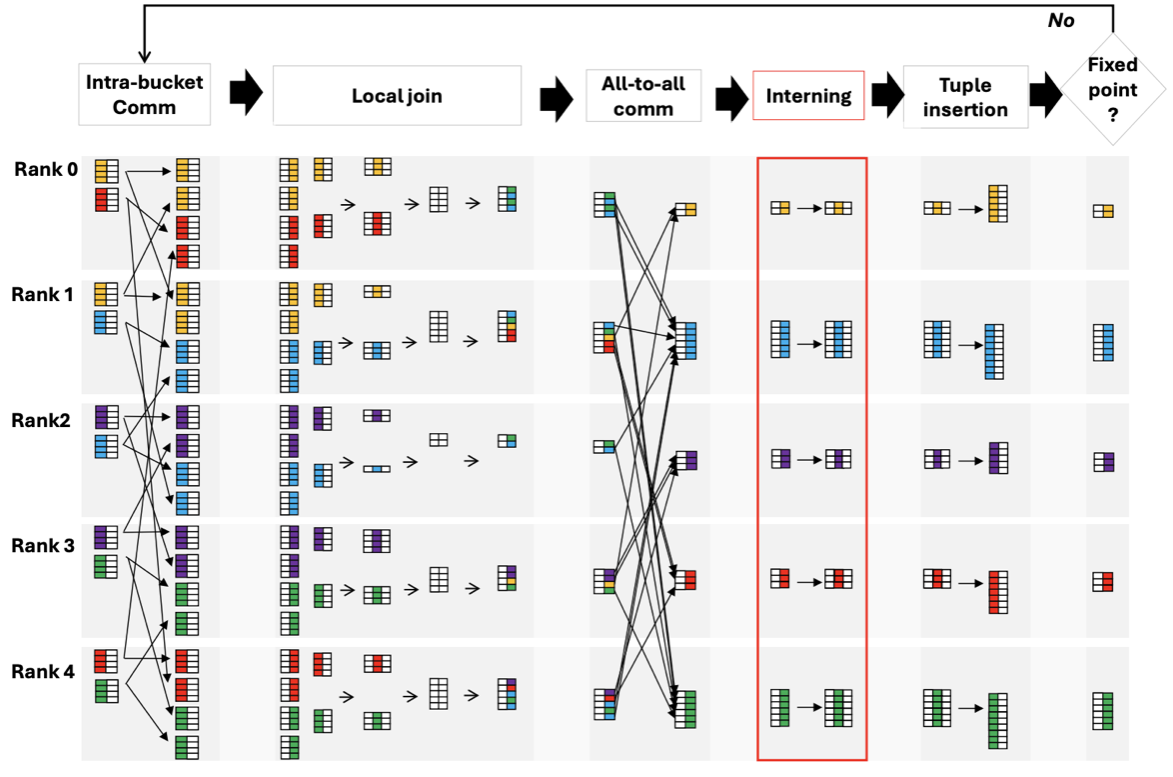
\includegraphics[width=0.55\textwidth]{JoinIteration.png}
  \vspace{-0.75cm}
  \caption{\footnotesize The major phases of one parallel-RA iteration.}
  \label{fig:bpra}
  \vspace{-0.5cm}
\end{wrapfigure}
%
My collaborators and I followed this up with an ISC paper presenting techniques to \emph{dynamically} balance an RA workload across iterations, both spatially and temporally---work awarded the \textbf{Hans Meuer \emph{best paper} award in 2020}. 
%
Figure on right shows a schematic diagram of the major phases
of our algorithm in the context of (an incrementalized) transitive closure computation. There are three primary phases of the system: (1) local, parallel RA computation, (2) all-to-all data exchange, and (3) interning, local insertion, and a fixed-point check. To maintain the distributed hash table for a subsequent fixed-point iteration, our algorithm requires an all-to-all data exchange with unusual characteristics compared to typical MPI algorithms. The data transfer is low-volume and moderately variadic, but has strict latency requirements as this is the only major synchronization point in the algorithm. With my PhD student Ke Fan and collaborator and co-advisor Sidharth Kumar, we developed a novel two-phase variant of the Bruck algorithm to optimize our all-to-all step, yielding good scaling for our workloads on up to about 8K processes on the Theta supercomputer. \textbf{Our novel variadic Bruck algorithm was published at HPDC 2022 and a version with tunable radix was published at ISC 2024}.  
Aspects of this work predated my PPoSS Planning grant, and was supported by a Directors Discretion grant from ALCF. To date I have used \textbf{over 5M hours on Theta} through this program. My work on parallel RA has been featured in the ALCF's annual \emph{Science Report} magazine\footnote{\url{https://www.alcf.anl.gov/sites/default/files/2021-04/ALCF_2020ScienceReport.pdf} (page 37)}.

In the last few years, my efforts in this direction have centered on GPUs and GPU-based clusters. My students, collaborators, and I have developed \textbf{three closely related GPU-based systems for relational algebra, published at ASPLOS 2025, and AAAI 2025, and ICS 2025, that all yield far superior performance on a single H100 versus 512 threads on ALCF's Theta} supercomputer, and show linear scaling for an approach that supports multi-node, multi-GPU joins. My PhD students and I are now investigating extensions for leveraging vectorized joins and worst-case-optimal joins.


\paragraph{Tunable Static Analysis}
%
My primary motivation for improving deductive reasoning systems has been to automate verification and optimization tasks in compilers for high-level functional and logical languages, and support related program analysis tasks for security auditing and reverse engineering. The heart of such problems lies in how to tune static analyses to achieve the necessary precision for relevant program behaviors while reigning in complexity to an acceptable degree so the analyses are practical for their target applications (flow-directed inlining, auditing information flow, property verification, etc).
%
Simulations of code that aim to approximate all possible program behaviors ahead of runtime are up against the halting problem and the fundamental limitations of computability: no particular style of compromise between precision and complexity will ever guarantee an analysis to be both effective and terminating. Instead, \textbf{a best-effort approach must permit the analysis to be flexibly tuned, while guaranteeing reasonable bounds on both correctness and complexity}. Ideally, it will permit bootstrapping analysis intelligence from simple coarse bounds on behavior that are easy to compute (such as context-insensitive control-flow and basic-type recovery) toward more granular, sophisticated, and context-sensitive program properties (such as shape analysis, refinement types, and symbolic path conditions).

To this end, I have developed a general approach to polyvariant and context-sensitive analysis that is easily tuned, by adjusting a policy for abstract heap allocation, while \textbf{guaranteeing soundness for all possible tunings}. This means analysis sensitivies may be tuned to optimize for effective precision only, as \textbf{soundness-by-construction is always guaranteed}---a framework \textbf{published at ICFP 2016}. This work also lead to an \textbf{invited follow-up} paper in the Journal of Functional Programming (JFP 2018). I surveyed a wide range of sensitivities to show that instrumenting analyses, to increase available information with which to tune polyvariance, allows me to demonstrate generality. The guarantee of soundness my framework provides permits directly introspective notions of polyvariance, with powerful ramifications.

For example, a long-standing problem in context-sensitive program analyses has been how to model the call stack so-as to ensure precise call-return matching as polyvariance is increased, with more complex approches using Dyck reachability at a substantial increase in complexity, among other proposals. Using my general framework for polyvariance, I was able to show that \textbf{perfect call-return matching can be achieved at no asymptotic increase in analysis complexity} (and a practical decrease in runtimes) with a simple introspective choice of continuation allocator. This result was \textbf{published at POPL 2016 and provided a mechanized proof of precision} using a bisimulation with an incomputable model (using an unbounded stack) that I implemented in the Rocq/Coq theorem prover. In the future, I will explore new approaches to autotuning and optimizing the polyvariance of program analyses to discover custom sensitivities that will enable verification of currently intractable program properties.

\paragraph{Gradual Verification}

Naturally, there will always be unsolvable problems in program verification and my highest ambition in this space is not to solve unsolvable problems but to unlock general and gradual approaches that permit greater practical capacities for verification while gracefully degrading to static warnings and reasonable runtime semantics in the worst-case. To this end, I have explored analysis of faceted execution, a paradigm for policy-agnostic programming (i.e., infosec policies)---publishing a novel analysis at CSF 2020. I have also worked on gradual approaches to contract verification that permit substantial static verification without user annotation by applying \textbf{abstract symbolic execution---a novel combination of symbolic execution applied to an abstract interpretation} developed with collaborators. Both of these approaches use a dynamic monitor that enforces key program properties at runtime, but which can be safely removed, or partially removed, in cases of successful static verification.  

\begin{wrapfigure}{l}{0.5\textwidth}
  \vspace{-0.50cm}
  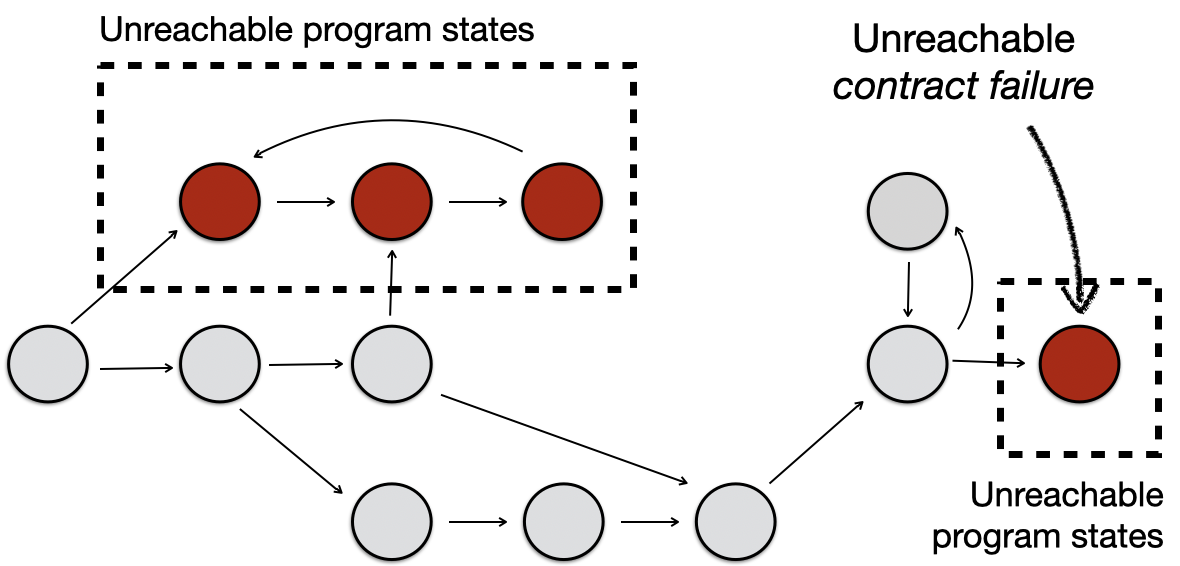
\includegraphics[width=0.5\textwidth]{ContractVerification.png}
  \vspace{-0.25cm}
  %\caption{\footnotesize A overapproximate control-flow graph wi}
  \label{fig:bpra}
  \vspace{-0.45cm}
\end{wrapfigure}
%
Symbolic execution associates program states with path conditions: SMT formulae that must hold at those program states. When applied to an overapproximate abstract interpretation, unsatisfiable path conditions strongly imply unreachable sets of program states. When these states encode contract failure, this effectively verifies the contract and permits its safe removal. I have \textbf{published an effective technique at POPL 2018 for verifying all but $28$ of $49,\!861$ dynamic checks} in a benchmark suite of stateful functional programs using this approach.
Collaborators and I then extended this approach by showing that a dynamic monitor of non-termination, using the size-change-termination principle, could be overapproximated and verified to yield proofs of totality---\textbf{work published at PLDI 2019}.    


\paragraph{Research Community}

I plan to serve the broader Datalog, declarative/logic programming, and program analysis communities by helping to standardize and disseminate open source tools, portable languages, and interfaces to improve the outreach of our work into practice and to accelerate research in related areas. To this end, \textbf{I am currently organizing a Datalog Modulo Theories Working Group} with Kris Micinski at Syracuse University and Max Willsey at UC Berkeley, bringing in several others working on applications and related techniques with the goal of standardizing portable interfaces and benchmarks for the mutual benefit of all researchers working in this space.
I seek to build collaborative networks of distinct supporting perspectives to pursue research goals that cannot be achieved by just one narrower vision acting alone. In my broader professional and service roles, I invest in developing my communities so all members can participate in this kind of collaborative innovation in a sustainable manner.  

I plan to further serve my research community by developing a workshop that can bring together researchers working on high-performance systems and declarative languages for reasoning and analysis. In 2019 I was invited to speak at the Workshop on Declarative Program Analysis (DPA), which was a wonderful event in this space. I met the founder of Semmle (later aquired by Microsoft's GitHub) and had some fascinating discussions with him and a few others. Unfortunately, this workshop has not been held since and I would like to either pick up the baton on running DPA or start a similar event with a mission to bring together researchers working on high-performance declarative \emph{reasoning} systems more broadly.

In 2019, I served as \textbf{program committee chair for the Scheme Workshop (SW)}, organizing a series of refereed and invited talks. This workshop was always special to me as the venue that first accepted my own work and gave me a chance to cut my teeth at academic writing and speaking as a new graduate student in programming languages. I met several of my long-term colleagues through the Scheme Workshop and want to continue supporting it.
I have also served on NSF panels, reviewed for journals TOPLAS and TCBB, served workshops like DLS and MiniKanren, and served several major conferences including on the ICSE PC, the POPL ERC, and the ECOOP AEC. 

\paragraph{Local Community}

Here at WSU I have served on qualifying exam and thesis committees, and on the hiring committee, conducting initial Zoom interviews and helping to focus our department's search for new faculty on the best possible candidates.
I am eager to hold service roles like these in the future and to be involved in building community both within my department and university. 

While at UAB, I ran the annual UAB high-school programming contest (HSPC) every year.
Our annual programming contest brought together students from nine regional secondary schools to compete in solving a set of programming challenges. I always enjoy working with undergrads to generate a set of fun and challenging problems for these guests that encourage out-of-the-box thinking. It's always impressive to me how successfully many of the high-school-aged competitors face such difficult problems. It's beautiful how the modern accessibility of computing hardware and knowledge permits talent to shine out so unmistakably, regardless of nominal background and resum\'e line items. I would like to run a similar event here at WSU, in collaboration with our student ACM organization.

As faculty sponsor to UAB's student ACM/ACM-W organization, who put on the HSPC and many other community events, I had an opportunity to help foster a positive and inclusive social environment for our students by running hackathons, leetcode nights, board-game nights, and an ``undistinguished'' lecture series where students practice their communication skills by presenting on non-research-related topics of personal interest such as archery, history of dance, blockchain technology, TempleOS, and Bollywood.

I also mentor students outside of computer science on how to leverage programming in their research. Sometimes simply automating data processing workflows with Python scripts and regular expressions, or SQL queries, have made a big difference for students in biology and medicine. When traveling to HiPC 2023, in India, I volunteered as a mentor to the Student Research Symposium. I also taught 3 sessions of introductory programming to grades 6, 7, and 9 at the local \emph{Diksha School} while there. I have frequently volunteered to speak with members of the broader public on topics related to my expertise. I've been interviewed by local press, and have appeared twice on ABC's \emph{``Talk of Alabama''} morning show\footnote{\url{https://tinyurl.com/abc-talk-of-alabama-gilray}}, once for a live interview and once for a live panel discussion with industry leaders on the impact and future of AI. 




\end{document}
